\begin{savequote}[75mm]
Nothing in Biology Makes Sense Except in the Light of Evolution
\qauthor{Theodosius Dobzhansky}
\end{savequote}

\chapter{Introduction}
\label{introduction}
\begin{flushleft}
\setlength{\parindent}{7ex}
\section{Disclosure}
Parts of this introduction, have been adapted from own publications, including \textit{Wnt signaling in cancer} \citep{zhanWntSignalingCancer2017} and \textit{The drug-induced phenotypic landscape of colorectal cancer organoids} \citep{betgeDruginducedPhenotypicLandscape2022}.

\section{Colorectal Cancer}
Colorectal Cancer is among the three most common and lethal forms of cancer in the developed world, accounting for ca. 10\% of all cancer incidence and mortality \citep{sungGlobalCancerStatistics2021}. The majority of colorectal cancer cases are diagnosed after the age of 50, are located in a region spanning the rectum and sigmoid colon, and develop from macroscopic precursor lesions referred to as adenomas over the course of ca. 10 years \citep{choGeneticAlterationsAdenoma1992}. Next to patient age, a sedentary lifestyle including obesity, diabetes, consumption of red and processed meats, alcohol and smoking constitute risk factors \citep{sungGlobalCancerStatistics2021}. The disease is classified by the Union for International Cancer Control (UICC) into five stages ranging from \textit{carcinoma-in-situ} (patch of malignant cells that has not yet breached the basal lamina of the intestinal mucosa), to stages 1 (malignant cells have breached the basal lamina), stage 2 (malignant cells have spread beyond the large muscle layer surrounding the colon mucosa), stage 3 (malignant cells have spread to loco-regional lymph nodes), and stage 4 (metastatic disease) \citep{vancutsemESMOConsensusGuidelines2016a}.
\par

Among the most effective interventions to reduce the incidence and mortality of colorectal cancer is the removal of macroscopic lesions during preventative colonoscopy \citep{nishiharaLongtermColorectalcancerIncidence2013}. In case the disease has further progressed, therapeutic options include oncological resection coupled with adjuvant chemotherapy (available for UICC 2, recommended for UICC 3) based on the DNA replication inhibitors 5-Fluoruracil (5FU) and Oxaliplatin (FOLFOX). Additional treatment options exist for patient subgroups such as rectal cancer patients (neoadjuvant radiochemotherapy) and frail patients (5FU instead of FOLFOX for adjuvant chemotherapy). In case of metastatic disease (UICC 4) the treatment depends on molecular characteristics of the tumor. Commonly available options include (1) combination chemotherapy (FOLFOX or FOLFIRI) paired with anti-Egfr antibodies (Cetuximab) for $KRAS$ wildtype disease \citep{vancutsemESMOConsensusGuidelines2016a}, (2) triple therapy (FOLFOXIRI \citep{vancutsemESMOConsensusGuidelines2016a}, or combined Egfr-, Mek- and Braf-inhibitor treatment \citep{kopetzEncorafenibBinimetinibCetuximab2019}) for $BRAF$ mutant disease, or (3) PD-1 immune checkpoint inhibition (Pembrolizumab, anti-PD1) for tumors with microsatellite instability (MSI+) \citep{andrePembrolizumabMicrosatelliteInstabilityHighAdvanced2020}. Therapeutic options can be combined with angiogenesis inhibiting therapeutic antibodies (Bevacizumab, anti-VEGFR), especially when patients are not able to undergo a full treatment regiment. Additional lines of therapy can also include agents like Regorafenib and Triflouridin/Tipiracil \citep{vancutsemESMOConsensusGuidelines2016a}. 
\par

\section{Colorectal Cancer Pathogenesis}

\subsection{The colon crypt}
The sequence of molecular events leading to colorectal cancer, or any cancer in general, are governed by the tissue's stem cell biology \citep{cleversCancerStemCell2011}. The colon stem cell niche, or crypt, is the source of all epithelial cells lining the colon. Similar to the small intestine, Lgr5+ intestinal stemcells are located at the bottom of the crypt and continuously renew the epithelium by proliferating and, through displacement, pushing newly formed cells towards the colon's lumen. This architecture serves multiple purposes, including protection of stem cells and the control of cell fate decisions across the epithelium \citep{cleversIntestinalCryptPrototype2013a}. Multiple developmental pathways, especially Wnt signaling, Notch, Bmp and RAS-MAPK signaling, govern cell identity and growth rate in the intestinal niche \citep{hTalesCryptNew2019}. The concentration of ligands for most of these signaling pathways is organized in gradients along the crypt-lumen axis. For example, the concentration of stem cell identity maintaining Wnt ligands (Wnt signaling) and growth-rate controlling Egf ligands (RAS-MAPK signaling), decreases as cells are pushed outside of the crypt \citep{sasakiReg4DeepCrypt2016}. In contrast, the effect of Bmp ligands, which promote cell differentiation, increases as the concentration of BMP inhibitors (i.e. Noggin) derived from basal mesenchymal cells decreases \citep{heBMPSignalingInhibits2004}. As a cell is pushed outside the crypt by a continuous stream of proliferating cells, the signals it receives and with it its gene expression changes - leading to cellular differentiation. Similarly, if enterocyte-progenitors are moved back into the crypt, the ambient signaling leads to a de-differentiation towards an intestinal stem cell state \citep{tettehReplacementLostLgr5Positive2016a}. \par

Given the spacial confinement of growth- and stemness-stimulating signals, the crypt architecture also leads to a protection against tissue damage. At the bottom of the crypt, a neutral competition of proliferating intestinal stem cells leads to the removal of damaged cells that show a reduced proliferation rate relative to population of surrounding stem cells \citep{snippertIntestinalCryptHomeostasis2010a}. Given this neutral competition and the dependence on external signals to proliferate, dysfunctional or transformed cells have a higher likelihood of being removed from the niche unless they acquire a set of molecular alterations that render them independent from niche signals and increase their growth rate. \par

\subsection{The adenoma carcinoma sequence}
Cancer in general, and colorectal cancer in particular, is a disease marked by the accumulation of genetic events in somatic cells, which over time lead to uncontrolled growth and spread beyond the tissue of origin. Both structural and functional genomics experiments have helped identify functional genetic events or "drivers", that cause the transition from controlled to malignant cellular state. A classic model for the sequence of functional events leading to colorectal cancer is known as the adenoma-carcinoma sequence \citep{vogelsteinGeneticAlterationsColorectaltumor1988}. It starts with the activation of the Wnt signaling pathway through loss of the tumor suppressor $APC$ and is followed by the activation of the RAS-MAPK signaling pathway through mutations of the $KRAS$ or $BRAF$ oncogene. Further mutations activating PI3K signaling (i.e. $PI3K$ oncogene, $PTEN$ tumor suppressor) and inhibiting Tgf-beta (i.e. $SMAD4$ tumor suppressor) and p53-signaling (i.e. TP53 tumor suppressor) complete the transformation from adenoma to invasive carcinoma \citep{fearonMolecularGeneticsColorectal2011}. \par

When simplified, colorectal cancer forms along the adenoma-carcinoma sequence through (I) a common chromosomal instability (ca 80\%) or (II) a DNA-mismatch repair deficiency (ca. 20\%) associated mechanism \citep{markowitzMolecularOriginsCancer2009} and \citep{pancioneGeneticEpigeneticEvents2012}. These two trajectories of tumor development have been associated with characteristic clinical, pathological, and molecular properties. 
\par

Tumors of the common chromosomal instability phenotype present themselves early as common, non-serrated polyps in the rectum and sigmoid colon \citep{markowitzMolecularOriginsCancer2009}. Most tumors are microsatellite stable and have frequent $APC$ truncating mutations coupled with KRAS activating mutations. 
\par 

In contrast, tumors of the DNA-mismatch repair phenotype are frequently present as serrated polyps and more likely to be located in the right colon \citep{markowitzMolecularOriginsCancer2009}. These tumors are often marked by a CPG-island methylation phenotype (CIMP) that can lead to the hypermethylation of tumor suppressors and DNA-mismatch repair genes \citep{oginoCpGIslandMethylator2009}. Consequently, these tumors have a higher proportion of microsatellite instability, higher mutational burden, higher immunogenicity, and thus a higher immune-cell infiltration. APC mutations are less frequent and if present more likely to be missense than truncating \citep{borowskyRoleAPCWNT2018}. Mutations of the BRAF oncogene are more frequently found than KRAS mutations. 
\par

Independent of the mechanism, the sequential accumulation of functional genetic events renders colorectal cancer cells progressively independent of the organism's tissue control mechanisms and thus enable the uncontrolled, independent growth of cells which defines late stage cancer.

\subsection{The role of APC and KRAS during colorectal cancer pathogenesis}
Genetic alterations in the tumor supressor $APC$ and the proto-oncogene $KRAS$ are among the two most frequent mutations found in colorectal cancer \citep{markowitzMolecularOriginsCancer2009}. Alterations in the two genes are highly correlated and found already at early stages \citep{minaConditionalSelectionGenomic2017}. What defines the interaction between the two colorectal cancer drivers, is, however, still an open question \citep{parsonsWNTDriverDependency2021}. In the following section the mechanism of Wnt signaling and ERK-MAPK signaling are briefly introduced, as these two pathways are directly affected by Apc loss and Kras activation, respectively, and both have a regulatory function within the colon stem cell niche \citep{hTalesCryptNew2019}.

\begin{figure}[h]
\centering
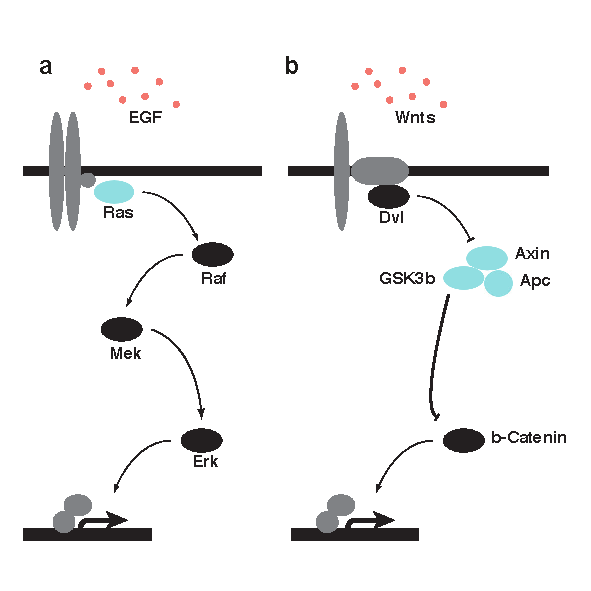
\includegraphics[width=0.55\textwidth,
                keepaspectratio]{figures/adenomaprofiling/pdf/fig_0_1.pdf}
\caption[Simplified illustration of ERK-MAPK signaling and canonical Wnt signaling]{\textbf{Simplified illustration of Egf dependent ERK-MAPK signaling and canonical Wnt signaling a} Egf dependent signaling cascade. Ras is highlighted in blue. \textbf{b} canonical Wnt signaling cascade. The destruction complex, including Apc, is highlighted in blue.}
\label{fig_180}
\end{figure}
\bigbreak

\subsubsection{canonical Wnt signaling during colorectal cancer pathogenesis}

Members of the Wnt signaling pathway were first identified as regulators of embryonic development \citep{sharmaEffectWinglessWg11976, nusslein-volhardMutationsAffectingSegment1980} and are controlling adult stem cell identity across tissues. As a result, members of the pathway are frequently altered during cancer initiation \citep{zhanWntSignalingCancer2017}. In canonical Wnt signaling, absence of Wnt ligands leads to phosphorylation of \textbeta-catenin by the destruction complex, which contains the scaffold protein Axin, the large disordered protein Apc (Adenomatous polyposis coli, $APC$) and the kinases Gsk3\textbeta as well as casein kinase (Ck1\textalpha) (reviewed in Zhan, Rindtorff et al.\citep{zhanWntSignalingCancer2017}). 
In this state, \textbeta-catenin is phosphorylated by Gsk3\textbeta, ubiquitinated by \textbeta-TrCP and subsequently targeted for proteasomal degradation. In the absence of nuclear \textbeta-catenin, the transcriptional repressive complex containing TCF/LEF and transducing-like enhancer protein (TLE/Groucho) recruits Histone deacetylases to repress target genes. \par 

The role of Wnt signaling during colorectal cancer development is well established \citep{polakisManyWaysWnt2007}. Here, loss of APC is the most frequent driver of Wnt signaling in colorectal cancer and can be found in about 80\% of colorectal cancer patients \citep{fearonMolecularGeneticsColorectal2011, zhanWntSignalingCancer2017}. Both in-vitro experiments with human colon organoids (introduced below) and genetic mouse models have demonstrated that loss of function of $APC$ ($Apc$ in mice) is sufficient to cause adenoma formation \citep{moserApcMinMouseModel1995}, which is marked by Wnt-ligand independent proliferation \citep{matanoModelingColorectalCancer2015a, Drost2015SequentialCells}. Further, $Apc$ is a necessary but not sufficient to sustain invasive tumor progression of in-vivo cancer models harboring additional functional events in $Kras$ and $Trp53$ \citep{dowApcRestorationPromotes2015a, sakaiCombinedMutationApc2018a}.
\par

\subsubsection{ERK-MAPK signaling during colorectal cancer pathogenesis}

The extracellular-signal-regulated (ERK) mitogen-activated protein kinase family (MAPK) is one of three major MAPK families, together with the JNK (c-jun N-terminal kinase or stress-activated protein kinases) and MAPK14 group of protein kinases \citep{zhangMAPKSignalPathways2002}. These signaling cascades play a major role in (I) integrating external proliferative signals, (II) reacting to stress or ambient cytokines and (III) protecting cells from apoptosis, respectively \citep{fangMAPKSignallingPathways2005}. The ERK-MAPK signaling cascade itself is constituted by a set of protein kinase subfamilies, Ras (encoded by i.e. $KRAS$, $NRAS$, $HRAS$), Raf (encoded by $BRAF$, $CRAF$, $ARAF$), Mek (encoded by $MEK1$, $MEK2$) and Erk ($ERK1$, $ERK2$) which transmit extracellular mitogenic stimuli in a step-wise signaling cascade towards transcription factors. \par

In the colon crypt, the ERK-MAPK signaling cascade and its members are key regulators of cell proliferation and tissue growth rate \citep{hTalesCryptNew2019}. Blockade or removal of Egf, a canonical ligand of the signaling cascade's upstream receptor (encoded by $EGFR$), leads to a cell cycle arrest of proliferating Lgr5+ cells while not affecting their cellular state \citep{basakInducedQuiescenceLgr52017}. As a result, Lgr5+ cells can re-enter proliferation as soon as ERK-MAPK signaling is restored.
\par

In colorectal cancer, the Ras kinase subfamily members are mutated in about 36\% of cases \citep{fangMAPKSignallingPathways2005}. Next to Ras, Raf mutations can also be found in around 10\% of colorectal cancers \citep{fangMAPKSignallingPathways2005}. Of note, mutations of $KRAS$ and $BRAF$ occur mostly in a mutually exclusive pattern (introduced above) \citep{fangMAPKSignallingPathways2005, minaConditionalSelectionGenomic2017}. According to the Vogelstein model of colorectal cancer initiation \citep{fearonMolecularGeneticsColorectal2011}, activating mutations of $KRAS$ takes place early during cancer development, more specifically, after loss of $APC$. In-vivo mouse models of the oncogenic $Kras^{G12D/+}$ show that this functional event is not sufficient to cause adenoma formation, but instead leads to $Cdkn2a$-dependent oncogene-induced senescence \citep{benneckeInk4aArfOncogeneinduced2010}. In the context of in-vivo $Apc$ loss of function ($Apc^{\Delta716}$), however, the $Kras^{G12D/+}$ genotype leads to an increased number of adenomas and reduced survival. Of note, the combination of $Apc$ loss and oncogenic $Kras$ in colon epithelial cells are not sufficient to cause invasive and metastatic disease in-vivo \citep{sakaiCombinedMutationApc2018a}, which is only seen in triple mutant genotypes (i.e. $Apc^{\Delta716}, Kras^{G12D/+}, Tgfbr2^{-/-}$) \citep{sakaiCombinedMutationApc2018a} 


\section{Organoids}

\subsection{Isolation of Culture of Organoids}

Organoids are three-dimensional cell culture models from primary adult tissue. Intestinal organoids develop from Lgr5+ adult stem cells and were first isolated from the small intestine of mice \citep{satoLongtermExpansionEpithelial2011}. Subsequently, following the initial publication, further organoid models across tissue-types and species have been developed. These include organoids from intact and cancerous human large intestine \citep{satoLongtermExpansionEpithelial2011}, pancreas \citep{driehuisPancreaticCancerOrganoids2019}, mammary epithelium \citep{zhangEstablishingEstrogenresponsiveMouse2017, sachsLivingBiobankBreast2018} and the hepatobiliary system \citep{huchVitroExpansionSingle2013}. The number of tissues that can be modeled through organoids has been continuously increasing since the first publication of this methodology. \par

Culturing organoids from primary cells requires the addition of specific tissue-dependent growth factors and the embedding of cells in 3D hydrogels \citep{merkerGastrointestinalOrganoidsHow2016}. In the case of colon organoids, the necessary growth factors are inspired by signaling cues available in the intestinal stem cell niche (discussed above): Wnt and R-spondin ligands to activate and maintain canonical Wnt signaling; EGF ligands to stimulate ERK MAPK signaling, and Noggin ligands to inhibit the differentiating effects of the BMP signaling cascade \citep{satoGrowingSelforganizingMiniguts2013}. When combined with inhibitors of TGF\textbeta and p38 mediated signaling, these growth factors enable organoid formation and continous proliferatation ex-vivo. In line with the niche-focused model of colon cancer formation outlined previously, patient derived colorectal cancer organoids proliferate in simpler conditions that correspond to their genetic state (i.e. $APC$ mutant colon organoids grow in conditions lacking Wnt and R-spondin ligands) \citep{Fujii2016-ax}. Not only the high isolation efficiency of up to 80\%, but also the high genetic and transcriptomic correlation with their tissue of origin have made organoids increasingly popular translational research model \citep{pauliPersonalizedVitroVivo2017a}. Both the high isolation efficiency, and the molecular representation of the tissue of origin are likely a result of the culture conditions which are mirroring the tissue-specific stem cell environment. These conditions reduce biases and evolutionary bottlenecks on the tissue's cells during the transfer into an in-vitro environment. \par

\subsection{Diagnostic use of Colorectal Cancer Organoids}

Given the benefits of the methodology, patient derived organoids are being trialed as predictive models for personalised treatment recommendation in colorectal cancer care \citep{vandeweteringProspectiveDerivationLiving2015, vlachogiannisPatientderivedOrganoidsModel2018, ganeshRectalCancerOrganoid2019, ooftPatientderivedOrganoidsCan2019a, yaoPatientDerivedOrganoidsPredict2020a}. In these assays, personalised organoid models are generated and then treated with a candidate drug in-vitro. While robust reports on the predictive validity of organoids for progression-free survival are still missing, current results for response rate models show noteworthy predictive validity for Irinotecan, FOLFIRI, and neoadjuvant radiation therapy. A pooled analyses of the previously published literature recently summarised the aggregate sensitivity and specificity for organoid based treatment response rate prediction at 0.81 and 0.74, respectively (conservative single-point AUROC estimate: 0.78) \citep{wensinkPatientderivedOrganoidsPredictive2021, zhangNoteROCAnalysis2005}. Despite the potential of patient derived organoids to guide clinical decision making, the method is not ready for use in a clinical context with a high biopsy-to-evaluation dropout rate and turnaround time being the primary technical hurdles. A recent failed single-arm prospective clinical trial for organoid-based last-line treatment recommendations reported a treatment for 6 out of 61 included patients (>90 \% dropout rate and 10 week turnaround time, 23 lost during organoid establishment, 11 lost due to disease progression) \citep{ooftProspectiveExperimentalTreatment2021}. Further improvements of reagents, isolation procedures, and in-vitro protocols might lead to lower dropout rates and turnaround times to enable further investigation of organoid-based diagnostics for personalised colorectal cancer care. \par

\subsection{Therapeutic Discovery using Colorectal Cancer Organoids} 

Next to diagnostics, organoid have been evaluated as models in drug discovery. Patient derived organoids can be processed in high-throughput small molecule screens with conventional, ATP-based, cell viability readouts \citep{vandeweteringProspectiveDerivationLiving2015}. In addition, besides testing therapeutic candidates on patient derived models, organoids are amenable to efficient genetic engineering using CRISPR \citep{matanoModelingColorectalCancer2015a, drostUseCRISPRmodifiedHuman2017}. This opens up the possibility of evaluating the effect of therapeutic candidates against precisely defined genetic disease states.

\section{Profiling Experiments} 

Profiling experiments are biological experiments in which high dimensional phenotypes are observed of biological models that are subjected to multiple treatments. Examples for such methods include Transcriptome Profiling Experiments (i.e. Perturb-Seq \citep{dixitPerturbSeqDissectingMolecular2016}, L1000 Profiling \citep{subramanianNextGenerationConnectivity2017}) as well as Image-based Profiling Experiments \citep{caicedoApplicationsImagebasedProfiling2016} (described below). These data intensive experiments generate three-dimensional data containing (1) multiple features (i.e. transcript count or morphological feature) for (2) multiple treatments (i.e. small molecules) and (3) multiple experimental units (i.e. multiple genetically perturbed cell lines, multiple organoids from different patients). The presence of high dimensional phenotype information for multiple treatments is what separates profiling experiments from observational studies, such as single-cell RNA-Sequencing of multiple untreated tissue samples (multiple features and multiple experimental units, but not multiple interventions). 

\subsection{Image-based Profiling}

Image-based profiling is an unbiased high-throughput microscopy based profiling method in which in-vitro models are systematically treated with small molecules or genetic perturbations (i.e. siRNA) to observe their treatment-induced phenotype \citep{caicedoApplicationsImagebasedProfiling2016}. A hallmark of image-based profiling is the emphasis on capturing unbiased morphological information from treated cells. In contrast to screening experiments which are focused on one particular phenotype of interest, image-based profiling experiments are using general purpose staining protocols (i.e. DNA, Actin, Mitochondria, and the cellular membrane). Given the large amount of collected information from such experiments, analysing their results is a common challenge and subject of continuous method development \citep{chandrasekaranImagebasedProfilingDrug2021}. 
\par

The image-based profiling method has previously been used in functional genomics research \citep{billmannGeneticInteractionMap2016} and translational biomedical research \citep{gibsonStrategyIdentifyingRepurposed2015}. While the exact approaches in which image-based profiling is used in each of these areas differ, a set of common steps exist: (1) Image Analysis, (2) Phenotype Modeling and (3) Novelty Detection. During Image Analysis, raw microscopy images are processed using manual or learnt feature extraction methods to generate a low-dimensional representation of each treatment-induced phenotype. Ideally, such representations are comparable across contexts, captures biological differences, and suppresses technical artefacts. Examples for different methods include classic texture feature calculations followed by Principal Component Analysis (PCA) \citep{caicedoDataanalysisStrategiesImagebased2017} as well as modern approaches such as end-to-end self-supervised learning with a contrastive-loss \citep{perakisContrastiveLearningSingleCell2021}. During Modeling, a set of conditions that are well annotated are observed and the low-dimensional representations of their treatment-induced phenotypes are modeled as a function of these treatment conditions. For example, the phenotype of siRNA treated Drosophila cells has been modeled as an effect of two combined siRNAs using a linear model \citep{billmannGeneticInteractionMap2016}, and the phenotype of small-molecule treated human cells has been modeled as an effect of a single disease allele using a boosting-based model \citep{gibsonStrategyIdentifyingRepurposed2015}. During Novelty Detection, a set of treatment conditions of interest are identified based on their deviations from the learnt model. For example, the phenotype of Drosophila cells might change more drastically than anticipated under a linear model after treatment with two siRNAs which target genes in the same signaling pathway (indicating a form of epistasis) \citep{billmannGeneticInteractionMap2016}. Analogously, a small-molecule induced phenotype of Human cells might be misclassified as wildtype, although the treated cells are bearing a disease allele (indicating a potential small molecule candidate inhibitor of the disease associated molecular mechanism) \citep{gibsonStrategyIdentifyingRepurposed2015}. Once identified, these novelties can be further validated in independent experiments to uncover new biological mechanisms or identify therapeutic candidates.
\par

\subsection{Matrix Factorization}
The basic goal of matrix factorization methods is to identify a small number of underlying factors within high-dimensional measured data that explain its intrinsic structure. 

\begin{equation}
    Y = ZW^T + \epsilon
\end{equation}

In this process, a data matrix \( Y \), consisting of \( n \) samples and \( m \) features, is decomposed into two lower-dimensional matrices: 

\begin{enumerate}
    \item The factor score matrix \( Z \), which has dimensions \( n \times k \), where \( k \) represents the number of latent factors. Each row in \( Z \) corresponds to a sample, and each column corresponds to a latent factor.
    \item The factor weight matrix \( W^T \), which has dimensions \( k \times m \). Here, each row corresponds to a latent factor, and each column corresponds to a feature. This matrix is also referred to as the loading matrix. 
\end{enumerate}

The factor score matrix \( Z \) can be understood as a learnt, lower-dimensional representation of the data with \( k \) dimensions. The choice of \( k \) (the number of latent factors) ideally strikes a balance between simplicity and comprehensiveness and can be algorithmically determined. 

Different matrix factorization methods exist, with Principal Component Analysis (PCA), non-negative matrix factorization (NMF) and Independent Component Analysis (ICA) being among the most common \citep{stein-obrienEnterMatrixFactorization2018}. Each of these methods performs the basic decomposition outlined above, but apply different constraints during the decomposition \citep{stein-obrienEnterMatrixFactorization2018}: In PCA the identified factors are orthogonal to each other and are ranked by the amount of variance they explain within the data. In NMF both the factor score and weight matrix must be non-negative, which aides interpretation. In ICA the factors are statistical independent and non-gaussian, which is useful for the analysis of time-course data, such as audio or electrical activity. Each of these three popular methods do not include further assumptions, such as a dedicated measurement error \(\epsilon\).

In case the data generating process is better understood and robust solutions are preferred, additional assumptions can be introduced. For example, directly modeling the measurement error for each feature \(\epsilon\) and applying sparsity constraints to the matrix factorization are options. If such additional assumptions are made, the method is more commonly referred to as a form of factor analysis \citep{klamiGroupFactorAnalysis2014}.


\subsection{Extending Matrix Factorization to multiple experimental Views}

Many physical processes of scientific interest can be observed through more than one method or "view". For example, a patient tissue sample can be characterised through DNA sequencing, RNA sequencing and lipid abundance measurements. Finding a small number of underlying factors across high-dimensional data coming from multiple views is thus an increasingly frequent problem in biological data analysis and is the focus of the multi-view representation learning field \citep{liSurveyMultiViewRepresentation2019}. In group factor analysis methods \citep{virtanenBayesianGroupFactor2012, klamiGroupFactorAnalysis2014}, which includes multi-omics factor analysis (MOFA, introduced further below) \citep{argelaguetMultiOmicsFactorAnalysis2018b, argelaguetMOFAStatisticalFramework2020a}, the factor analysis described above is extended to multiple data views (also referred to as modalities): A set of \(m\) data matrices \( Y_m \) is decomposed into a single factor score matrix \( Z \) and a corresponding set of \(m\) weight matrices \( W_m^T \) and error terms \(\epsilon_m\). 

\begin{equation}
    Y_m = ZW_m^T + \epsilon_m
\end{equation}

Factors that are identified using this approach describe patterns within the data that can span multiple different data modalities. Next to simplifying the interpretation of complex data, factors that have been learnt to represent the structure of measurements across multiple modalities with group factor analysis have been shown to enable more reliable similarity estimation and missing data prediction than alternative factor analysis methods or simply raw features taken from the measured data \citep{klamiGroupFactorAnalysis2014}.
\par

Multi-omics matrix factorisation (MOFA) builds on group factor analysis to learn a multi-view representation from data generated by omics-methods \citep{argelaguetMultiOmicsFactorAnalysis2018b, argelaguetMOFAStatisticalFramework2020a}. While other methods, such as classical group factor analysis, can be used to learn a representation across multiple modalities, MOFA has been developed with design choices that make it particularly useful for complex biological data:

\begin{enumerate}
    \item feature sparsity - the model reduces the number of features assigned to a given factor
    \item factor sparsity - the model reduces the number of factors that are assigned to a given modality
    \item modality-specific priors - the model uses dedicated priors for continuous, binary and count-based modalities 
    \item missing data handling - the model can be trained on incomplete observations
    \item speed - the model is fast to run compared to alternative methods, such as group factor analysis
\end{enumerate}
 
\bigbreak
In the context of the work presented in this thesis, multi-omics factor analysis (MOFA) is used to learn multi-modality representations for both patient derived and genetically engineered colon organoids. The modeled data comprised modalities such as organoid morphology, transcript expression, protein, and lipid abundance. The identified factors correspond to major axes of biological variation and help in the interpretation of results from image-based profiling experiments as outlined below. 

\subsection{Using Matrix Factorization to guide decision making}

While matrix factorization methods are commonly used to learn the intrinsic structure of high-dimensional data within an exploratory context, it can also be used to guide decision making by predicting similarities between observations. In the latter context, a well-annotated subset of the data, here referred to as the support set, is first used to learn factors. In a second step, another set of observations which are to be investigated, here referred to as query set, are projected into the learnt representation to estimate their properties. The "support set" and "query set" terminology is adapted from the field of meta-learning - a part of the machine learning literature focused on scenarios when only few well-annotated observations are available \citep{hospedalesMetaLearningNeuralNetworks2020}, a common situation in biomedical research and therapeutic discovery. 
\par

In order to estimate the factor scores for new observations in the query set the previously identified factor weight matrix is used. 

\begin{equation}
    Z_{\text{new}} = Y_{\text{new}} W^+
\end{equation}

Instead of decomposing the query data matrix \(Y_{\text{new}}\) into a factor score matrix and factor weight matrix, as done during the initial learning, the query data matrix  \(Y_{\text{new}}\) is multiplied with an approximated inverse of the factor weight matrix \( W^+ \) to estimate the corresponding factor scores \( Z_{\text{new}} \).
\par

In practice, scenarios in which such a multi-step approach is applied include sequential decision making problems, for example recommender systems \citep{korenMatrixFactorizationTechniques2009}. Here, a new observation is added to a set of existing observations to inform the best next action (i.e. an experiment to run, or a product to recommend). In this thesis a related approach is used for multi-view profiling of in-vitro organoid models. This approach is useful especially when cost differences between data modalities exist and treatment conditions with an effect of interest are rare: Instead of observing and modeling all possible treatments with multiple views at once (i.e. transcript expression, morphology, protein abundance), a representative subset, the support set, is first selected and fully observed to learn a multi-view model. This subset includes well annotated conditions, such as untreated in-vitro models of healthy and diseased tissue. In a second step, a large number of treatment conditions, the query set, are observed with only one modality. This modality is affordable and sufficiently informative (i.e. microscopy images). In the third and final step, the single-view observations are projected using the previously defined multi-view model. Provided the support set was representative enough, treatment conditions that show an effect of interest (i.e. the observed phenotype deviates from the expectation) are identified as novel and can be further characterised by gathering observations from additional views as well as running additional independent experiments.

\newpage
\section{Aims of Thesis}

Organoids are high fidelity three-dimensional in-vitro models that can be generated from cancer and normal tissue. Both advanced and early stages of colorectal cancer can be effectively modeled using Organoids. To model advanced stages of the disease, patient derived cancer organoids can be isolated from biopsy samples, which represent their tumor of origin both in terms of molecular features and morphology \citep{pauliPersonalizedVitroVivo2017a}. To model the earliest stages of the disease, the ability to culture organoids derived from healthy colon tissue and genetically engineer them using CRISPR allows the step-wise construction of colorectal cancer precursor states in-vitro \citep{matanoModelingColorectalCancer2015a, drostUseCRISPRmodifiedHuman2017}. Previously, in-vitro small molecule sensitivity tests of organoid models have been performed in diagnostic and in a translational research contexts \citep{vandeweteringProspectiveDerivationLiving2015, vlachogiannisPatientderivedOrganoidsModel2018, ganeshRectalCancerOrganoid2019, ooftPatientderivedOrganoidsCan2019, yaoPatientDerivedOrganoidsPredict2020}. 
\par
Image-based profiling is a high-throughput microscopy based method to systematically describe treatment-induced phenotypes of in-vitro models and has been used in translational research and therapeutic discovery contexts \citep{caicedoApplicationsImagebasedProfiling2016}. Despite its potential, the method has not -until recently- \citep{betgeDruginducedPhenotypicLandscape2022} been used to profile organoid models of colorectal cancer.
\par

\begin{figure}[h]
\centering
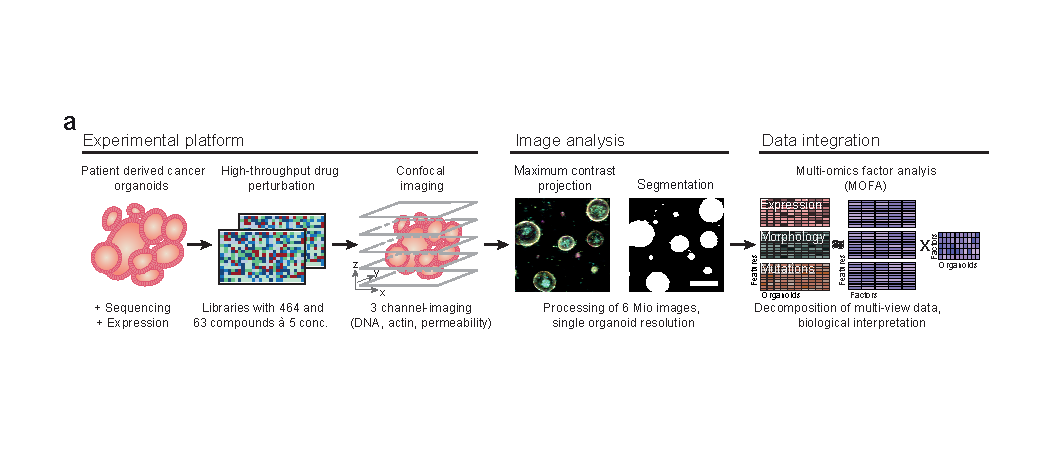
\includegraphics[width=\textwidth,
                height=\textheight,
                keepaspectratio]{figures/promise/pdf/fig_1_1.pdf}
\caption[Overview of organoid multi-view profiling experiments]{\textbf{Overview of organoid multi-view profiling experiments} Organoids were a) isolated from endoscopic biopsies from patients with colorectal cancer or b) derived from mouse samples and modified using CRISPR and conditional allele expression. Organoids were dissociated and evenly seeded in 384-well plates before perturbation with small molecules (ca. 800 and 1600 conditions for patient derived and mouse organoids, respectively). After treatment, high-throughput fluorescence microscopy was used to capture the morphology of organoids.  The multi-channel (DNA, beta-actin, cell permeability) 3D imaging data was projected, segmented, and descriptive features were extracted to quantify potential drug-induced phenotypes. Untreated organoid morphology, organoid size and drug activity scores were integrated with additional modalities, such as mRNA expression and DNA sequencing data in a Multi-Omics Factor Analysis (MOFA) to increase interpretability of organoid variation. Figure adapted from \textit{The drug-induced phenotypic landscape of colorectal cancer organoids} \citep{betgeDruginducedPhenotypicLandscape2022}}
\label{fig_130}
\end{figure}

This thesis introduces image-based profiling for colorectal cancer organoid models. The method is used to understand multi-omics factors of variation in 11 patient derived and 4 engineered organoid models with wiltype, $Apc^-/-$, $Kras^{G12D/+}$, and $Apc^-/-, Kras^{G12D/+}$ genotype. To summarise, the three central aims of this thesis are:
\begin{enumerate}
    \item Establish and perform image-based profiling for patient derived and engineered colorectal cancer organoid models.
    \item Understand primary multi-omics factors of molecular and morphological heterogeneity in patient derived colorectal cancer organoids as well as their influence on small molecule treatment sensitivity differences.
    \item Understand the degree to which image-based profiling of genetically engineered mouse colon organoids can recover known multi-omics molecular hallmarks of early colon cancer pathogenesis as well as genotype-specific small molecule treatment sensitivity differences.
\end{enumerate}


\end{flushleft}